\section{Coses a saber abans de començar}

\subsection{Notació dels Moviments}

El cub de rubik es resol gràcies a identificar patrons i executar algoritmes que resolen aquests patrons, aquests algoritmes han d'estar escrits en alguna part per poder-los memoritzar i per això estaà la notació del cub de rubik.
\\\\La notació consta de 6 moviments (F,B,R,L,U,D), que correspon a (Front, Back, Right, Left, Up, Down) que son les respectives direccions en anglés. Per exemple si faig el moviment F gira la cara front la que està més propera a la nostra visió, en sentit horari, en canvi si fós F' seria antihorari. En les figures següents es mostra una respresentació gràfica per a cada capa.
\\\\És un concepte difícil d'entendre però de manera simplificada és girar la cara en sentit horari i antihorari desde la cara que vulguis. En les figures següents es mostra una respresentació gràfica per a cada capa.

\begin{figure}[!ht]
    \centering
    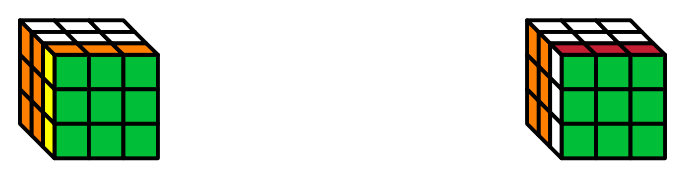
\includegraphics[width=7cm]{img/cubes/moviment-F.png}
    \caption{Exemples de Movimients F y F'}
\end{figure}

\begin{figure}[!ht]
    \centering
    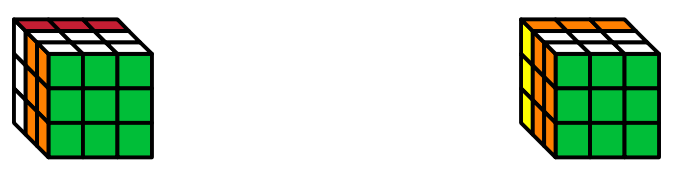
\includegraphics[width=7cm]{img/cubes/moviment-B.png}
    \caption{Exemples de Movimients B y B'}
\end{figure}

\begin{figure}[!ht]
    \centering
    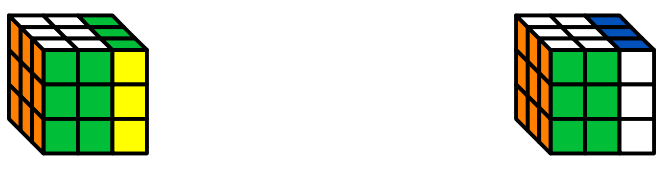
\includegraphics[width=7cm]{img/cubes/moviment-R.png}
    \caption{Exemples de Movimients R y R'}
\end{figure}

\begin{figure}[!ht]
    \centering
    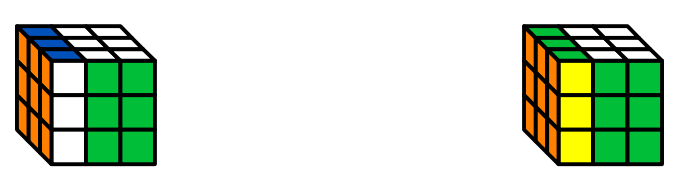
\includegraphics[width=7cm]{img/cubes/moviment-L.png}
    \caption{Exemples de Movimients L y L'}
\end{figure}

\begin{figure}[!ht]
    \centering
    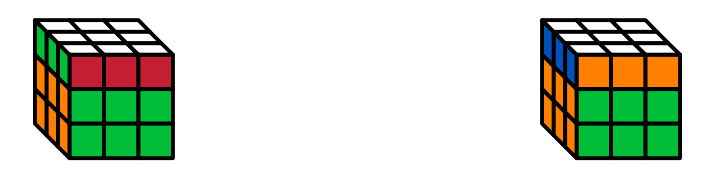
\includegraphics[width=7cm]{img/cubes/moviment-U.png}
    \caption{Exemples de Movimients U y U'}
\end{figure}

\begin{figure}[!ht]
    \centering
    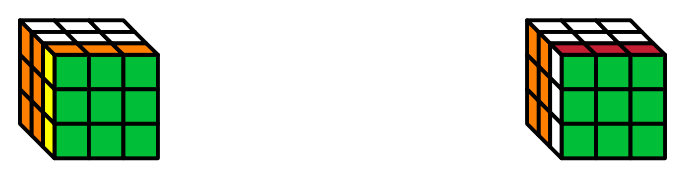
\includegraphics[width=7cm]{img/cubes/moviment-F.png}
    \caption{Exemples de Movimients D y D'}
\end{figure}

\subsection{Interpretar el concepte del cub}

La manera correcta d'interpretar el cub és pensar en el funcionament, com si el desmuntessis, ja que consta de 12 arestes i 8 cantonades, a més a més dels 6 centres que no poden permutar\footnote{Intercanvi de posició amb una altre peça i de l'ordre de tot el conjunt} amb cap altra peça ja que només roten.

\begin{figure}[h!]
    \centering
    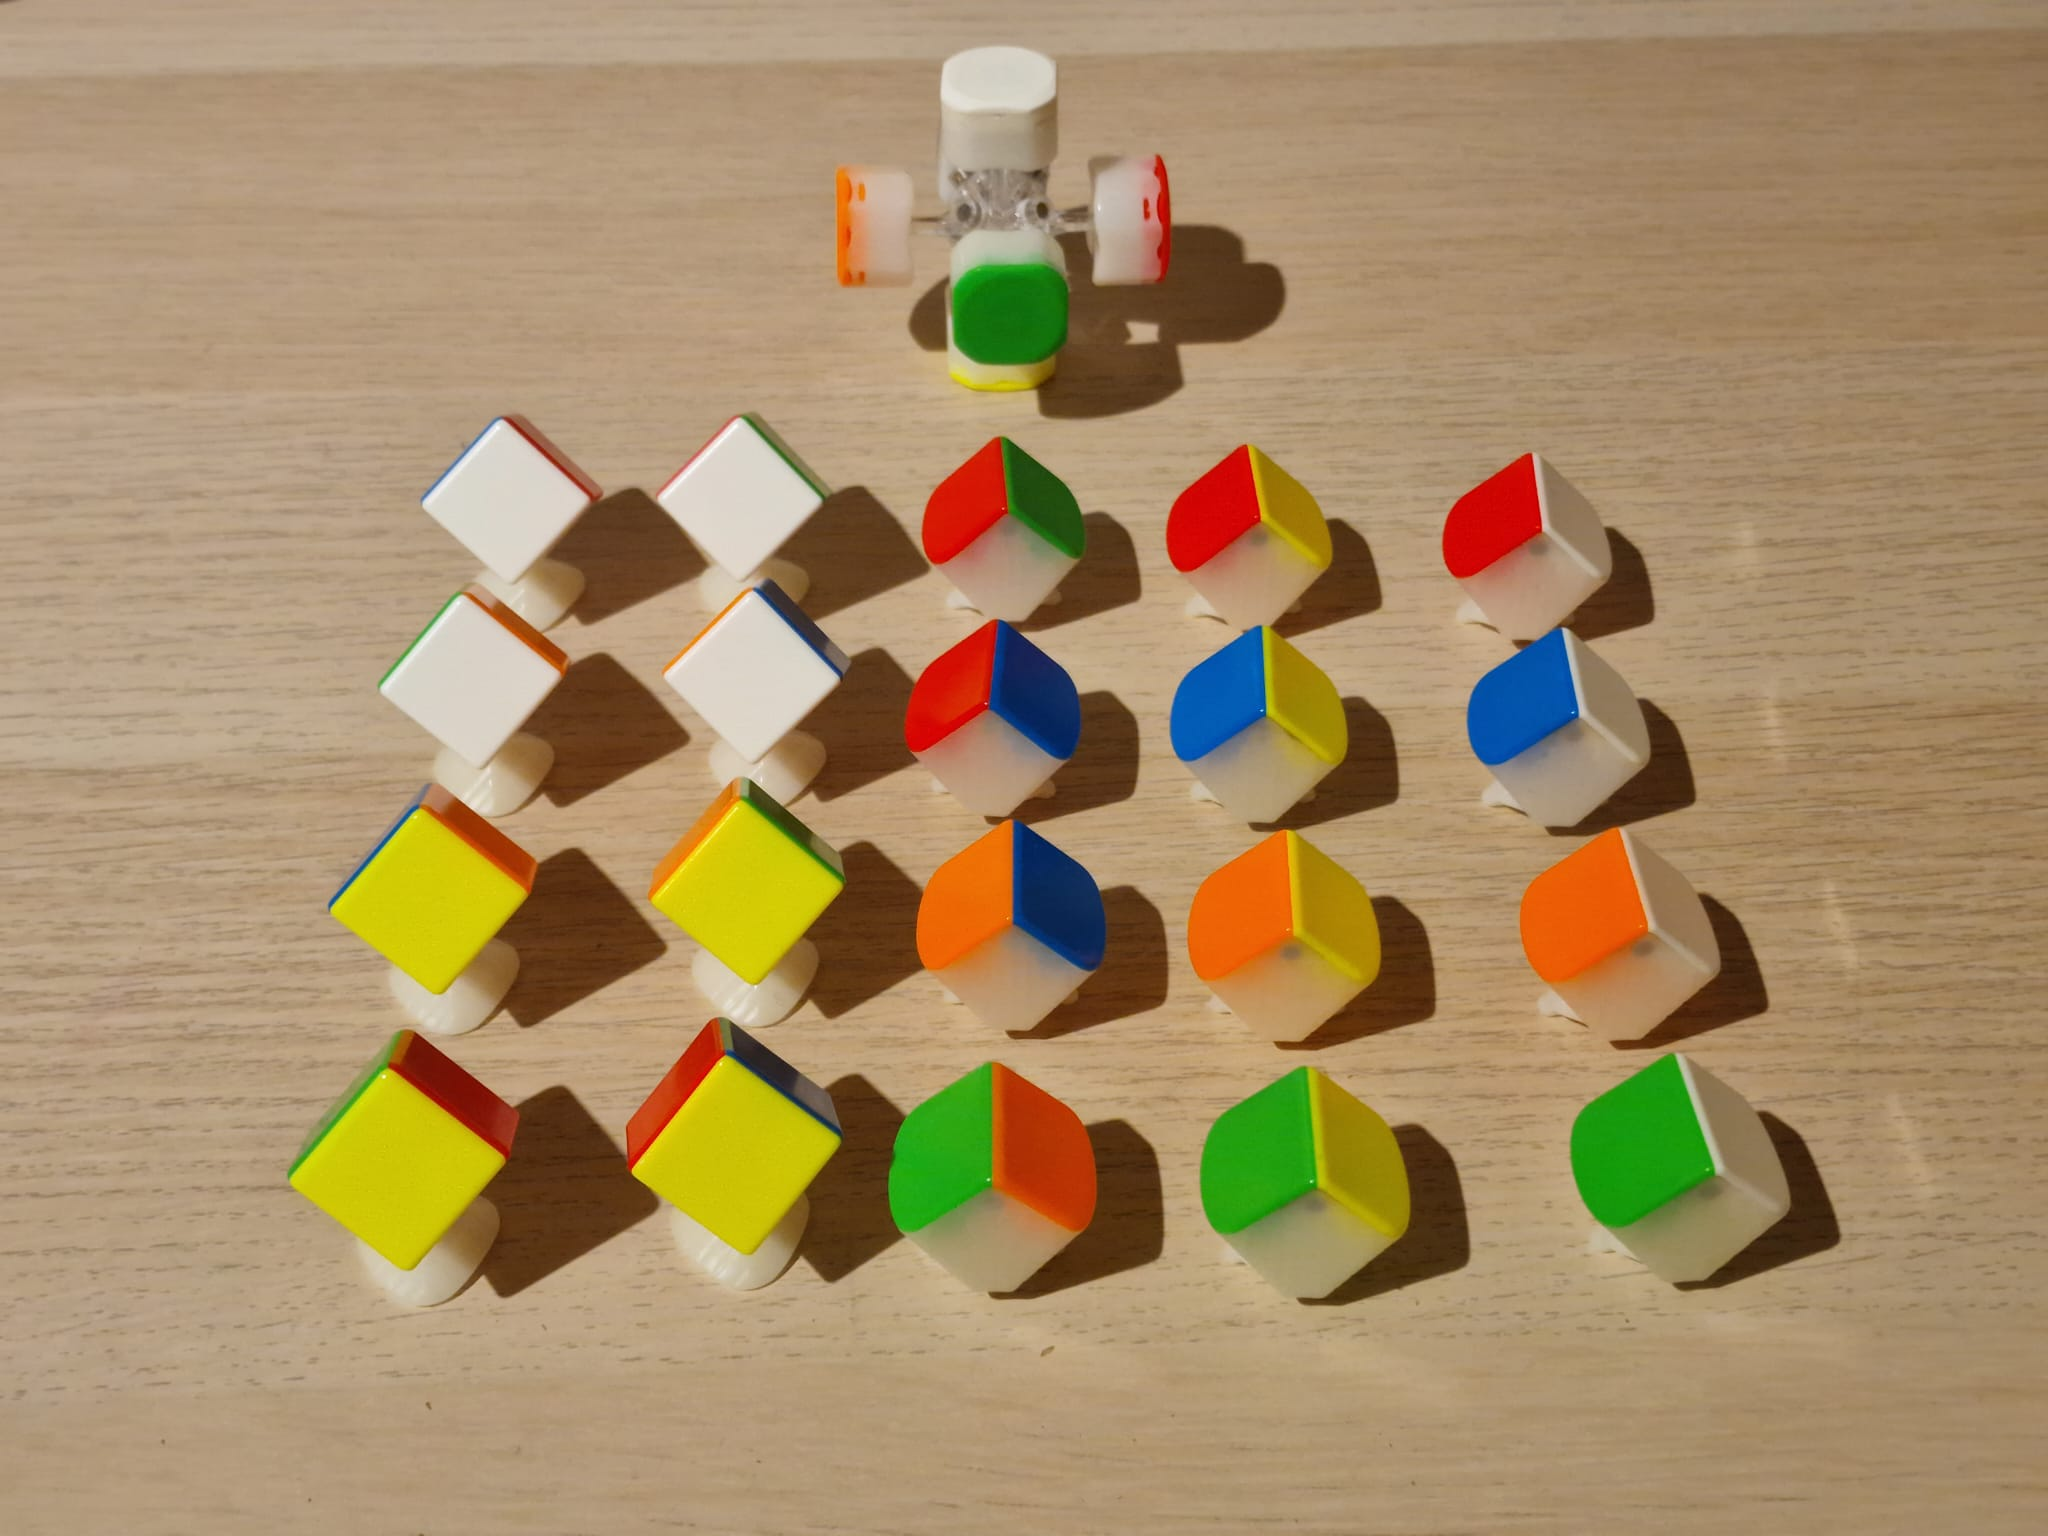
\includegraphics[width=7cm]{img/figures/cub-desmontat.jpg}
    \caption{Cub Desmuntat}
    \label{fig:cub-desmuntat}
\end{figure}
